\section{Problem \& Approach} \label{sect:overview}

\subsection{Problem Definition} \label{sect:problem}

We consider a data owner (client) storing her data in encrypted form on a server, possibly residing on a centralized cloud or a peer-to-peer (P2P) network.
The owner may run computational intensive tasks over the encrypted data.
Instead of performing on the server itself, the owner delegates the computational tasks to multiple workers residing on a decentralized cloud. 
Each worker fetches its portion of the required dataset from the server, performs the requested computation, and returns the results to the server.
The owner can then, at her discretion, download and verify the results.
The worker is financially rewarded if the verification of the returned results passes through.
This is illustrated in Figure~\ref{fig:model}.

\begin{figure}[h!]\centering
  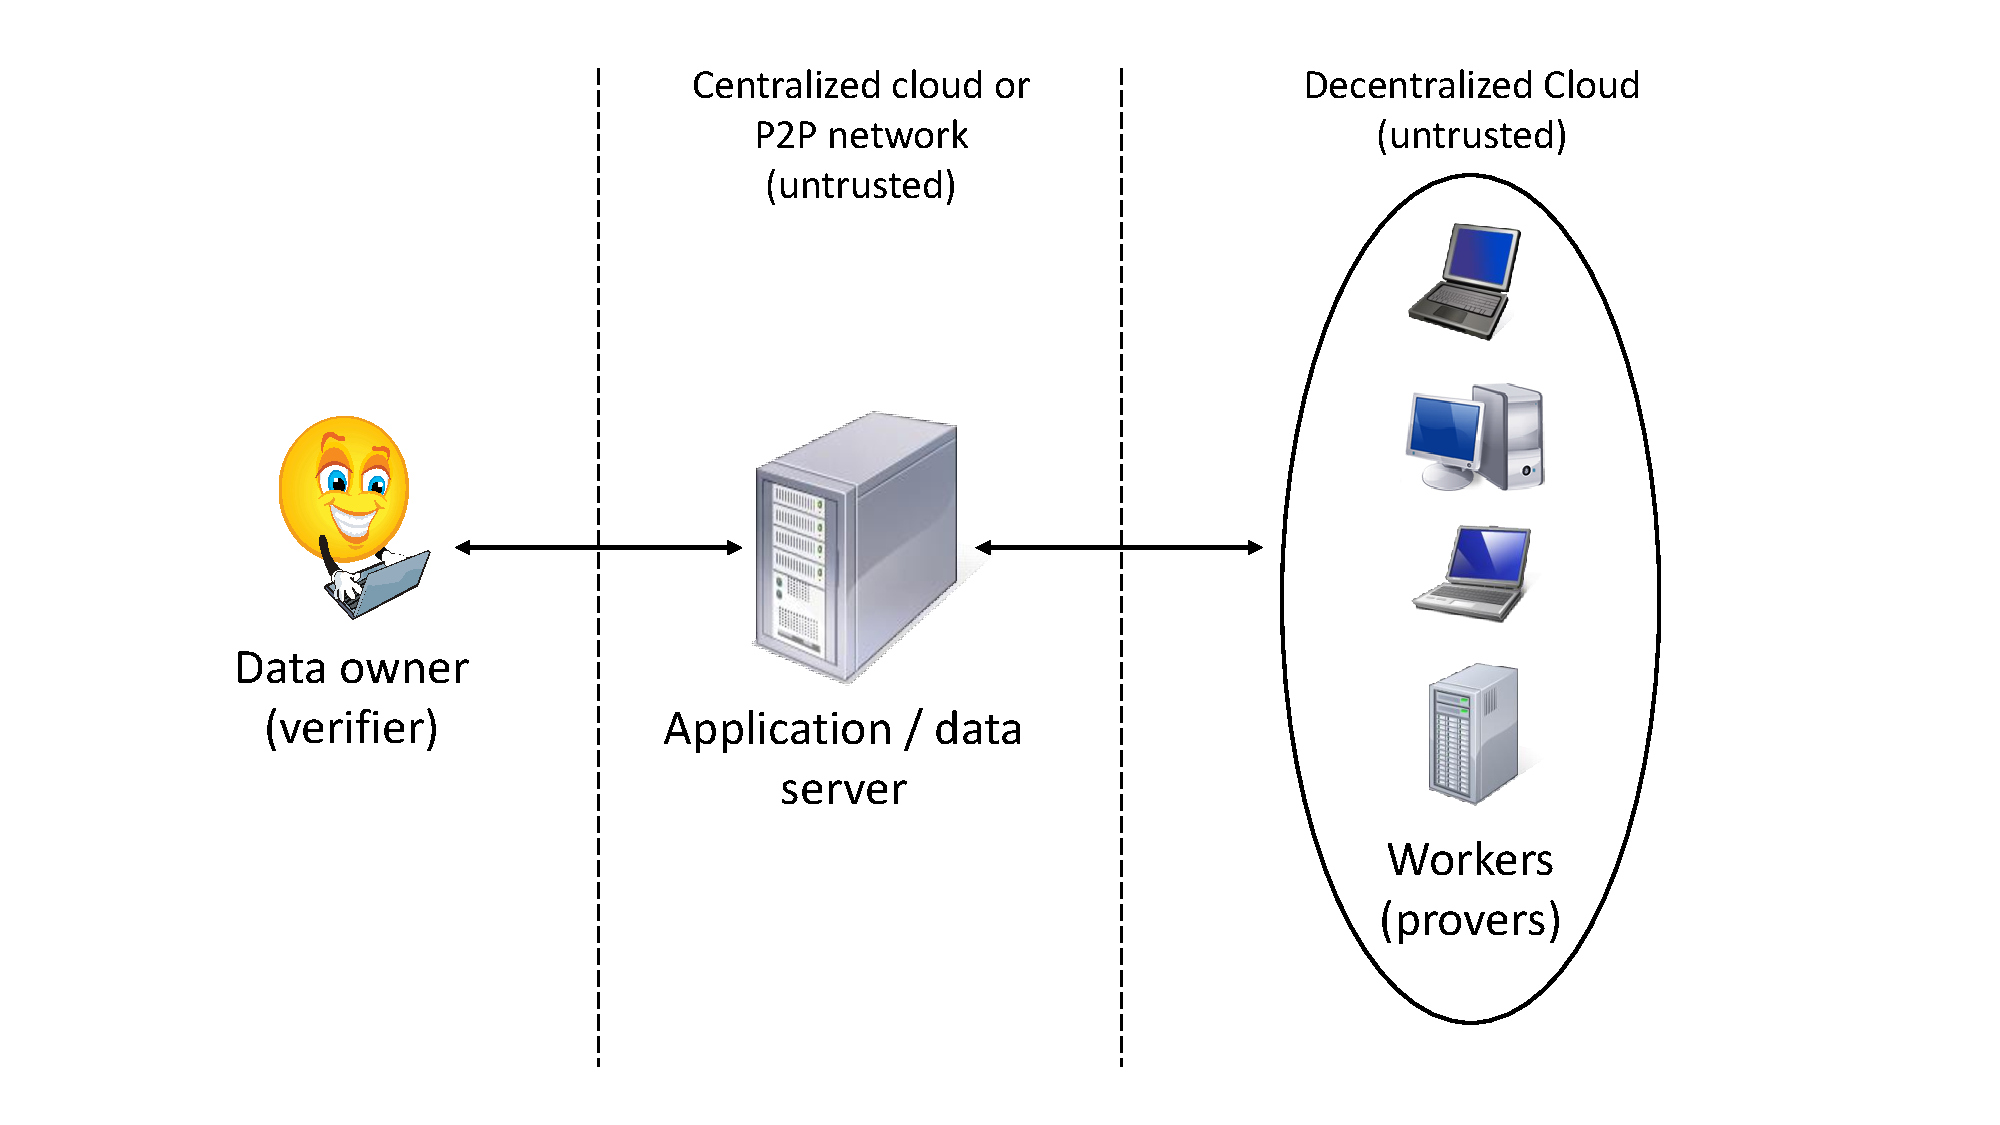
\includegraphics[scale=0.30]{model.pdf}
  \caption{Outsource of data and computation to a decentralized cloud.}
  \label{fig:model}
\end{figure}

\paragraph{Threat Model.}
However, each worker is assumed to be untrusted and they may deviate from the intended computation for various reasons, e.g., to save on computational cost. 
%It is essential, therefore, for the client to be able to verify the correctness of the computation. 
On the other hand, the worker may not trust the data owner either, in the sense that the worker may not be rewarded even if it has completed the computation and proved the correctness of the computation.


\subsection{Challenges} \label{sect:challenges}

\subsection{Solution Overview} \label{sect:solution}